\chapter{Model-View-Controller for Science}\label{chapter:MVC}

\section{Introduction}
Developing a computer program is much more than having few scripts that you can run when you need. A program should take care of a lot of concerns, such as the limits of the devices, should be flexible enough that enables you to change what measurements you are doing without spending months. More importantly, a program should be extensible in the long run, not just by yourself but also by future colleagues and, potentially, by anyone who find your program online. 

Therefore, when we develop software, we want to keep in mind the following programmer's \emph{mantras}:

\begin{itemize}
\item What you develop should be readable by current and future colleagues
\item It should be easy to add solutions developed by others
\item The program should allow exchanging devices that achieve the same goal (i.e. oscilloscopes of different brands, etc.)
\item The code developed in one context has to be available in other contexts (i.e. in other experiments)
\end{itemize}

The first line does not pose a challend to be understood. When we talk about solutions developed by others, we mean that often times someone already wrote a driver for a device, or they wrote a measurement script. Therefore, it should be easy to get other's code and use them in our own projects. Exchanging devices is something that is not valued until it happens. In most labs there is always a legacy device that sooner or later will break down and will need to be replaced. Or you move to a different lab and need to continue with your experiments with different hardware. We will see strategies in the program to allow easy exchange of devices. Finally, when we talk about context, we mean that sometimes experiments are very different, but the logic behind is very similar. We are measuring the I-V curve of a diode, but it is, by no means, any different from doing a 1-D scan on a confocal microscope, or tuning the wavelength of a laser. 

The mantras are not rules. They are just points on which you have to reflect in order to realize whether you are departing from the path you wanted to follow when you started. In the following sections we are going to explore a design pattern for software that has many benefits when developing scientific software for controlling experiments, it is called \textbf{The Model-View-Controller for Science}

\section{The MVCs design pattern}\label{section:MVC}
\begin{center}
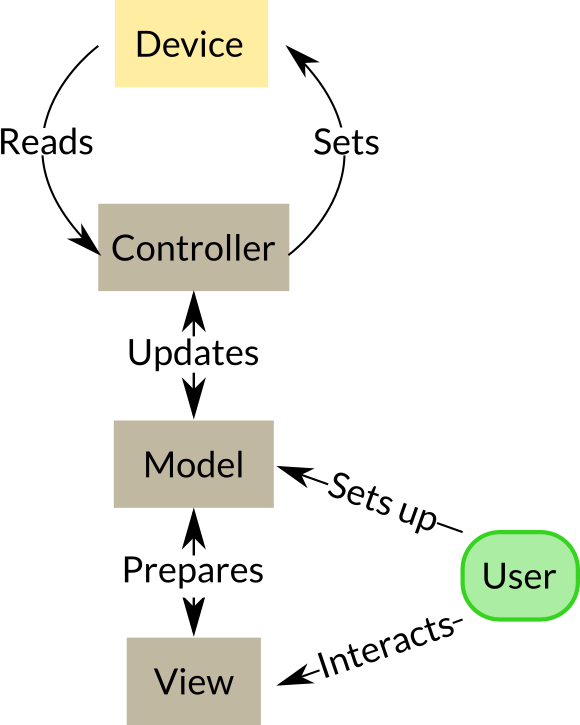
\includegraphics{images/Chapter_04/MVCs.png}
\end{center}

A design pattern is nothing more than a set of rules that determine where different parts of the code are going to be placed and how are they going to interact with each other. One of such patterns is called the Model-View-Controller, or MVC for short. When you work with devices in the lab, there is an extra layer that most computer programs lack, which is the interaction with the real world through specific devices. That is why we decided to nickname the pattern MVCs, with the s for \emph{science}. Let's see what each component of the MVC is about. 

A \emph{Controller} for our purposes can also be called \emph{a driver}, which is responsible for communicating with devices. It can be a Python class we developed ourself such as the one we did in the previous chapter, but it can also be a Python package developed by someone else. The latter scenario is the case when manufacturers provide the drivers themselves, such as PyPylons from Basler, or the NI-DAQmx bindings for Python. The driver has to reflect the capabilities of the device, nothing less and nothing more. For example, if a device is able to acquire just a data point at a time, the driver shouldn't include a function for acquiring an array of data using a loop. We briefly discussed this in the previous chapter. Whatever belongs to the logic that a user imposes belongs to Model component. 

The \emph{Model} is where all the logic is defined. In the models, we are going to define how we are going to use a device for our own experiment. A clear example would be the introduction of units. The device from the previous chapter takes only integer values as inputs. If we would like to transform that input to voltages, we could do it in the model for the device. Moreover, one of the analog  inputs is measuring a voltage, but it can be transformed to a current. This is very specific to our experiment and thus the option shouldn't be hardcoded in the driver. The place to include this information is the model. The main advantage of splitting \emph{Controllers} and \emph{Models} is that it becomes simple to upgrade or replace a device. You will need to update the \emph{Model} in order to reflect the new options of the device, but the logic of the experiment is left intact. 

There is a second type of model, which is the \emph{Experiment Model}, in which we link different devices in order to perform a measurement. Or we use a single device, but we add the features that an experiment needs, for example saving data, plotting, analysing, etc. With very simple examples, the boundary between the device model and the experiment model can be blurry, but when you are dealing with several devices or more complex flows, it becomes much clearer. At the end of the book we will give as a reference some projects we have worked on, that can be a good source of inspiration.

The \emph{View} is the place where you can locate everything related to how you show data to the user, and how the user can change the parameters of the experiment. In practice, it is the collection of files that build up a Graphical User Interface ({GUI}). Within the {GUI} you will set, for example, the start, stop, and step of the experiment. This information will be passed to the model to acquire the data. You can plot the results back to the user and save them to disk, etc. It is important to note that, in this case, the user interacts through the view with the model and never directly with the controller of a device. It is also important to keep in mind that all the logic of what you are developing should be implemented in the model. For example, if you save the data to files, the procedure to create new filenames should be specified in the Model and not in the View. 

For our project, the Controller is what we discussed on Chapter \ref{chapter:first-driver}

\warning{If you are new to developing code for the lab, it may seem that splitting \emph{Controller} and \emph{Model} is a waste of time. When
you have only one device that you use for only one goal, it may very well be the case. However, when you wish to include code developed by
others or when you want to share your code, it is crucial that you split the capabilities of your device from the logic of your experiment. If
you don't do so, all your code is going to work only when doing just one, very specific, experiment.}

You have to remember that the meaning of \emph{Model}, \emph{View} and \emph{Controller} changes depending on each developer or community. It
is important to note that people developing a web application are not dealing with devices in the real world as developers in the lab do. Therefore, how the {MVC} pattern is used can change from one field to another. Once you understand what each component is, you will very quickly understand where you need to change the code in order to solve a bug or add new functionality. 

\section{Structure of The Program}\label{structure-of-theprogram}
In the program you are developing in this book, you will follow the {MVC} design pattern quite literally. This means that you have to create
three folders called \emph{Model}, \emph{View} and \emph{Controller}. In the previous chapter, you have already developed the driver for the device. Go ahead and move the file \textbf{simple\_daq.py} into the Controller folder.

\exercise{Create a file \textbf{analog\_daq.py} in the Models. Inside the file, define a class called \mintinline{python}{AnalogDaq} and move the methods that you think appropriate from the Controller into the Model.}

In our definition of Model, it is important to make a further distinction. On the one hand, you have models for the devices that you use. In those models, you will define things such as units, how to initialize the device, etc. However, experiments often require to perform complex tasks in which several devices are synchronized. When you do an experiment you will need to save the data or load the configuration from a file. 

\exercise{Create a file in the Models folder, called \textbf{experiment.py}. Define a class called \mintinline{python}{Experiment} and add some methods that you think are going to be useful. You can, for example, add a method for switching on or off the {LED}. You can also add a method for doing a scan of an analog output signal. The methods can be empty, don't worry about making it work, but about the layout. You have to start thinking about the parameters that you need and the order in which every method can be called. For example, you can't save the data if you didn't perform any experiments.}

The View folder is going to require a bit more of work than the other two. However, you can already start thinking about how the user is going
to interact with your program. Most likely, you have already thought that sometimes the {LED} will be plugged into the output channel number 1,
sometimes to channel number 0. You don't want to change the code every time you change where you plugged the LED. The same happens, for example, with the channel you want to monitor, the time delay between steps, etc. All this behavior will be included in the view in the last chapters of the book. 

Now that you have started to split the code into different folders and files, it is important to discuss how can you make programs that use the code available in different files. That is called \emph{importing} and is the focus of the next section. 

\section{Importing modules in Python}\label{section:importing-python}
In the previous chapter, we have already seen some lines that look like this:

\begin{minted}{python}
import numpy as np
from time import sleep
\end{minted}

The first one is importing the numpy package, but changing its name to \mintinline{python}{np}. Changing the name makes it easier to work with because you need to type only two letters, \mintinline{python}{np} instead of \mintinline{python}{numpy}. The second line is importing one specific function from a package called \mintinline{python}{time}. It is important to realize that the import process was different in both cases. \emph{Numpy} is a complex package, with a lot of modules that can be used. The same is true for \emph{time}. However, in the lines above you have imported only the module \emph{sleep} from package \emph{time}. If you want to use it, you can simply do:

\begin{minted}{python}
sleep(1)
\end{minted}

While for using \emph{Numpy}, you will need to specify which module you want:

\begin{minted}{python}
np.random.random(1)
\end{minted}

If you know you only want to use \mintinline{python}{random} from \emph{Numpy}, you can also import and use it like this:

\begin{minted}{python}
 from numpy.random import random
 
 random(1)
\end{minted}

You may wonder why you would import all of numpy is you are just using one of its functions. The name \emph{random} is not defined solely by numpy. Python also provides its own random module. You can import it like this:

\begin{minted}{python}
 import random
\end{minted}

If you needed both \emph{random} functions in the same program, you would have a clash. How would you be sure you are using Numpy's and not Python's function? You may, for example, define your own random function and you would like to be able to choose which one to use and, more importantly, you want to avoid generating an unexpected behavior because of redefining functions without realizing it. 

When working with your own code, you can import different modules in the same way. Open a terminal and navigate to the root folder of the project, i.e. the folder that contains the Model, View, and Controller folders. Start the Python interpreter, and then type:

\begin{minted}{pycon}
>>> import Controller
\end{minted}

Now you have the controller available to use. For example, you can do the following:

\begin{minted}{pycon}
>>> dev = Controller.simple_daq.SimpleDaq('/dev/ttyACM0')
\end{minted}

And you can use the device as you have been using it in the previous chapter. Importing the \emph{Controller} may not be exactly what you
want, because sometimes there are many devices and you need only one. You can specify which module to import, exactly as you have done with
\mintinline{python}{from time import sleep}. To import only the SimpleDaq class, you can do:

\begin{minted}{pycon}
>>> from Controller import simple_daq
>>> dev = simple_daq.SimpleDaq('COM1')
\end{minted}

There are two things important to notice. First, if you change the code of the \emph{SimpleDaq} class and import it again, you won't see those
changes reflected. You should exit from Python and start again. The second thing is that, when you import the controller, you may also start
communicating with the device. This is happening because at the end of the \textbf{simple\_daq.py} file, you have added some lines for actually using
the class. Those lines also get imported and executed. When you import modules, and when you design modules, it is very important being in control of what is going to be executed. You don't want to trigger a measurement just because a user imported your driver. 

To avoid starting the communication with the device when you do \mintinline{python}{import simple_daq}, you have to add one line of code at
the end of the file. It will look like this:

\begin{minted}{python}
if __name__ == "__main__":
    d = SimpleDaq('/dev/ttyACM0')
    print(d.query('IDN'))
    d.write('OUT:CH0:4000')
    input('Press to read value')
    print(d.query('IN:CH0'))
    d.finalize()
\end{minted}

Next time you do \mintinline{python}{import simple_daq}, the code that follows the if statement will not be executed. However, if you run the file itself by typing \mintinline{bash}{python simple_daq.py}, it will. This is very useful because it allows you to distinguish the two cases, when the file is directly executed and when the file is imported. In many cases, you can use the bottom of the file to show how the class is used or to perform some quick tests. In the code above you can quickly see how to start the communication, query for the serial number, change the analog output, etc.

To understand a bit more about how the \mintinline{python}{if __name__} works and have a clearer picture of the importing procedure in Python, create
a new file called \textbf{dummy\_controller.py} in the \emph{Controller} folder, and paste the following lines of code:

\begin{minted}{python}
print('This is the dummy Controller')

def dummy_example():
    print('This is a function in the dummy Controller')

if __name__ == '__main__':
    print('This is printed only from __main__')
\end{minted}

From the terminal, enter into the Controller folder and type \mint{bash}|python dummy_controller.py| The output that you see should be:

\begin{minted}{python}
'This is the dummy Controller'
'This is printed only from __main__'
\end{minted}

What you see is that the entire code got executed but not the function itself. \mintinline{python}{dummy_example} is only defined, but never executed.

\exercise{What do you expect to happen if you do \mintinline{python}{import dummy_controller}?}

Things are going to be different when you import the file. Open the Python interpreter and type the following:

\begin{minted}{pycon}
>>> import dummy_controller
"This is the dummy Controller"
>>> dummy_controller.dummy_example()
"This is a function in the dummy Controller"
>>> from dummy_controller import dummy_example
>>> dummy_example()
"This is a function in the dummy Controller"
\end{minted}

The first thing you should notice is that what is written at the end never gets executed, meaning that the \mintinline{python}{if} statement is not
\mintinline{python}{True}. This is very useful when we want to have code that works standalone (when we execute it directly, for example) but we don't want to execute those lines if we import it. In the case of the real controller, we wanted to leave some examples at the end to show how it can be used, but when you are importing a class, you don't really want it to start communicating with the device.

The other thing that you should have noticed is that depending on how you import from a file, the first print statement is executed or not. If
you type \mintinline{python}{import dummy_controller}, you will see that the first print statement is there, while if you type \mint{python}|from dummy_controller import dummy_example| nothing happens. Python knows that you have already imported the module \textbf{dummy\_controller} and it doesn't execute again the lines that were already executed. This is very useful because it means that if you are developing a module that requires some setup, you can import it as many times as you need, knowing that the setup will be run only once. 

Finally, it doesn't really matter how you imported the dummy controller, the \mint{python}|dummy_example| function will always be available. It can happen that you either have to type \mintinline{python}{dummy_controller.dummy_example()} or simply \mint{python}|dummy_example()| but you will always see the same output. If you were sitting in an outer directory, you would have to do \mint{python}|Controller.dummy_controller.dummy_example()| and it would still work. When working with modules, there is plenty of flexibility on what to do. Bear in mind, however, that the same flexibility comes accompanied by some usage patterns that may not be clear.

Imagine you add a second function to your \mintinline{python}{dummy_controller.py} file, you can import both at the same time by typing
\mint{python}|from dummy_controller import dummy_example, second_function| You could also do \mint{python}|from dummy_controller import *| The
second option, however, is highly discouraged. There are several disadvantages to doing so. First, if you are reading the code and you
see something called \mintinline{python}{second_function} you have no idea where it came from. Also, if the \mintinline{python}{dummy_controller} creates variables, they will appear in your own program, perhaps overriding something you wanted to preserve.

\note{We should establish some naming conventions in order to avoid confusion later on. In Python, any file that defines variables, functions, classes, etc. is called a \mintinline{python}{Module}. The folder that contains modules is called a \mintinline{python}{Package}.}

Working with the imports in Python is sometimes easier than understanding them, especially when trying to pay attention to all the different definitions. The \href{https://docs.python.org/3.6/tutorial/modules.html}{Python Documentation} has a great chapter covering a lot of the ideas here
discussed. Many of the properties and behaviors can be learned by trial and error, though it can be very time consuming and it may lead to unexpected errors.

Perhaps you noticed by now that the way our package is imported and the way \emph{Numpy} is imported is very different. \emph{Numpy} can be
imported regardless of where you have started the Python interpreter. However, our package can only be imported if you are in its own directory. When you perform an \emph{import}, Python searches for modules in specific locations, and once it finds one, it stops searching. \emph{Numpy} is located in one of such folders, but your package is not. One of the ways in which you can let Python know where your package is located is by adding the folder of your package to a system variable called \emph{PYTHONPATH}.

If you are on Windows, you can follow the steps of Chapter 2, when you were dealing with the details of adding environment variables when
installing Python. If you are on Linux, it is enough to run the following command:

\begin{minted}{bash}
export PYTHONPATH=$PYTHONPATH":/path/to/PFTL"
\end{minted}

Remember that you have to change \texttt{/path/to/PFTL} with the full path to the folder where you are keeping your code. After doing that, you will be able to type \mint{python}|from Controller import *| wherever you are in your computer and Python will find the appropriate folder. In Linux, the change is not permanent, you will need to run the line again next time you start the Terminal. There are ways of modifying the environment variables in a permanent way, but it is up to you to find out. There are a lot of tutorials available online, according to your own distribution. 

Even if you are able to import your packages, there is still something important missing. It is standard that each package (i.e. each folder that contains modules) has an extra \textbf{\_\_init\_\_.py} file. In the simplest of cases, it can be an empty file. This will let Python know that the folder should be treated as a package with modules inside, preventing problems in case a package is called as a built-in module of Python. 

\exercise{Create a folder called \textbf{random} and inside put a new file called \textbf{test.py}. Define a function inside the file, it is not important what it does; then save it. Start Python and see what happens if you do \mintinline{python}{from random import test}. Quit the interpreter and add an empty file called \textbf{\_\_init.py\_\_} inside the \textbf{random} folder. Try to import \textbf{test} again and see what happens.}

The previous exercise shows you how important it can be to let Python know that a specific folder is a package. If you were developing numpy, you would like to be sure you are importing your own random module and not the built-in Python one. It is very hard to know all the built-in modules that Python has available. Some are common and thus you can avoid using the same name, but it may happen that you inadvertently used a name that clashes to something else. 

We have seen that an empty \textbf{\_\_init\_\_.py} file can be used to tell Python that a folder is a package. However, \texttt{\_\_init\_\_} files can do much more than that. Let's create an \textbf{\_\_init\_\_.py} file within the \emph{Controller} directory and add the following code to it:

\begin{minted}{python}
from .simple_daq import SimpleDaq

controller_variable = "var"

print("This is the init of the controller")
\end{minted}

Go back to the root folder, one level up from the Controller folder and start Python. Then, execute the following command:

\begin{minted}{pycon}
>>> import Controller
"This is the init of the controller"
\end{minted}

If you think about what you did and what you are seeing on the screen, you can realize that the \texttt{\_\_init\_\_} file is being executed when you imported the \emph{Controller}, that is why you see the line being printed to screen. But that is not all. If you want to use the \emph{SimpleDaq}
class, you can just do \mint{pycon}|>>> Controller.SimpleDaq(/dev/ttyACM0)|. Moreover, the \mintinline{python}{controller_variable} is also available after importing. You can see it by typing:

\begin{minted}{pycon}
>>> print(Controller.controller_variable)
"var"
\end{minted}

You could also import only the Controller class or the variable. You should just do:

\begin{minted}{pycon}
>>> from Controller import Controller_variable
>>> from Controller import SimpleDaq
\end{minted}

How many times do you see the print happening? Interesting, isn't it? Python takes care of executing the code only once, the first time it
encounters an import statement. We will look again at the \textbf{\_\_init\_\_.py} file later on. For the time being it is
important that you realize that sometimes some definitions happen within that file. Especially if you are looking at code developed by someone else, and you don't understand how the imports are working, you should then check the \texttt{\_\_init\_\_} files to try to see what they are doing. Remember that a lot of code can be executed within the \textbf{\_\_init\_\_.py} file and therefore you should also look into them when there is
something mysterious that you cannot understand.

\exercise{Read the \href{https://docs.python.org/3/tutorial/modules.html}{Python Documentation} and find a way in which the code \mintinline{python}{from Controller import *} imports only the \mintinline{python}{SimpleDaq} class and not the variable we introduced in the \texttt{\_\_init\_\_} file.}

\section{The Final Layout}\label{the-finallayout}
At this stage, you should have a clear separation of your code into Model, Controller, and View. Most of them are, for the time being, empty folders, but you should know from now on where each part of the program is going to be found. However, you are not limited to having only three folders in your project. Most likely you want to provide some examples of how to use your code, or some documentation for your package. You may want to use some files to hold configuration parameters, which could be inside of a \emph{Config} folder.

However, if you create extra folders next to the three main ones, the structure of the program will start to be polluted. It won't be clear what is part of the package, what is a user-specific setting, etc. Therefore, is common practice to make a folder structure in which you will separate what is the program, what are the examples, etc. Your folder structure will look like this:

\begin{minted}{text}
├── Docs/
├── Examples/
│   └── Config/
└── PythonForTheLab/
    ├── Controller/
    ├── Model/
    ├── View/
    └── __init__.py
\end{minted}

There are three folders at the top level: \emph{Docs}, \emph{Examples} and \emph{PythonForTheLab}. The last one is holding the \emph{Model}, \emph{View} and \emph{Controller} with all the code that you have developed up to now. The \emph{PythonForTheLab} also requires an \texttt{\_\_init\_\_} file, because it is our main package. If you followed the steps in order to add the folder where you are working to the PYTHONPATH variable, now you can do the following:

\begin{minted}{pycon}
>>> from PythonForTheLab import Controller
\end{minted}

We have also added a \textbf{Config} folder. When we perform experiments, there are going to be a lot of parameters involved. For example, you need to define which channel to use as an output and which one as an input. You may want to determine the delay time between one point and the next and the range for the scan. Having a separated place for defining all the parameters will give you a very quick overview of what things you need to take care of and it will give a clear roadmap for your code, as we will see in the following chapters. 

You may wonder why we have the \textbf{Config} folder inside the \textbf{Examples} folder. What you have to consider is that the program you are developing right now may be used by someone else, who has different configuration requirements than yours. Therefore, the user can use your configuration file as an example and adapt it to her needs. It can also happen that you want to run the experiment with different configuration parameters and you can put each configuration in a different folder, maybe organized day by day. Remember that we can now run the code from any place in our computer because Python knows where the folder \textbf{PythonForTheLab} is located. 

\subsection{The Configuration File}\label{subsection:configuration-file}
Before we keep developing code, we need to stop for a second to think what do we want our program to do. We need to think about what inputs are needed for our program. For example, we know we need the port in which the device is connected. We also know that we need to define an output and input channel, a range for the scan, a delay between data points, etc. Before going into the details, let's see how to easily store all these parameters into a text file. 

In the \emph{Config} folder, create a file called \textbf{experiment.yml}. This file will hold all the parameters of the experiment. We are going to use a format called {YAML}, which has a very simple structure, it looks like this:

\begin{minted}{yaml}
Experiment:
  name: This is a test Experiment
  range: [1, 10, 0.1]
  list:
   - first Element
   - second Element
\end{minted}

{YAML} is very simple to read both by a person and by the computer. It has just a few rules, the most important one is that the indentation is done with \textbf{2} spaces. In the example above, there is a main element called \textbf{Experiment}, everything that is indented compared to that element will belong to it. Save the file and let's see how you can read it with Python. The library that we are going to use to read these files is called PyYAML which was installed in Chapter \ref{chapter:setting-up}. 

\begin{minted}{python}
import yaml

with open('Config/experiment.yml', 'r') as f:
    e = yaml.load(f)

print(e['Experiment'])
for k in e['Experiment']:
    print(k)
    print(e['Experiment'][k])
    print(10*'-')
\end{minted}

We will discuss more about yaml files later on. For the time being it is important that you know how to start working with them. You first open the file using \mintinline{python}{open}. We use the \mintinline{python}{with} command because it is very handy for working with files and other resources that have the same pattern of opening/doing/closing. Yaml is responsible for interpreting the information contained in the file. We store this information in a variable \mintinline{python}{e}, which is a dictionary. 

The elements of dictionaries are addressed by keys. In the example above, there is a main key called \mintinline{python}{'Experiment'}, and the
sub-keys \mintinline{python}{'name'}, \mintinline{python}{'range'} and \mintinline{python}{'list'}. If you want to use
one of those elements, you can type \mintinline{python}{e['Experiment']['name']}, for example. The code above just prints out each element,
separated by a horizontal line. Note that yaml imported the file directly as a dictionary but some of the elements are special. You can see that \texttt{'name'} is a string, but \texttt{'range'} and \texttt{'list'} are not. This will become very handy later on because YAML automatically detects what kind of information we are using. 

\exercise{What type of variables has yaml generated for \texttt{'range'} and the \texttt{'list'}? (Remember that you can use \mintinline{python}{type(var)} to know the type of the variable.}

\exercise{YAML also supports numeric information. Create a new element and assign it a value of \texttt{1} or \texttt{3.14}. What kind of variable has YAML created in such cases?}

Of course, YAML can be used not only to read properties but also to save information generated in a program. Instead of loading data, you need to use the \mintinline{python}{yaml.dump} method. For example, you can define a dictionary with the following information

\begin{minted}{python}
d = {'Experiment': {
    'name': 'Name of experiment',
    'range': [1, 10],
    'list': (1, 2, 3),}
}
\end{minted}

If you want to save it to a file, we can do the following:

\begin{minted}{python}
with open('data.yml', 'w') as f:
    f.write(yaml.dump(d, default_flow_style=False))
\end{minted}

Pay attention that in the code above, when you open the file, you are using the \mintinline{python}{'w'} option. This means that every time you run the code, you will overwrite the file and lose the previous contents. After running the code, open the file \textbf{data.yml} with a text editor and explore its contents. You will see that it is very similar to the one you created yourself earlier. One of the advantages of YAML is that the files are very easy to read. If you explore the contents of \textbf{data.yml} you know immediately what it contains.

\exercise{Read back the contents of \textbf{data.yml} and check that they are the same you saved.}

\exercise{Modify some of the values of \textbf{data.yml} directly with your text editor and see that those changes are reflected when you read again the file.}

\exercise{Create a numpy array and store it using yaml. How does it look like in the file? What happens if you read it back?}

\exercise{\textbf{Advanced}. Save a numpy array using yaml. Then activate a virtual environment in which PyYAML is available but not numpy. Try to load the contents of the file. What happens?}

Now that you know how to work with YAML files, is time to start thinking about the experiment again. You need to stop and think about what do you need to know in order to perform an experiment. We are going to cover the details in the next chapter, but it is important that you really focus and try to do it on your own in order to understand how the config files can be of great help when you develop software for your lab. Try to complete the following exercise to the best of your possibilities.

\exercise{Create an experiment.yml file in the \emph{Config} folder. Use what you have learned about YAML files to write a file that contains all the information that you need to perform an experiment and interpret its data. For example, knowing \emph{who} performed an experiment may be important.}

\subsection{Loading the Config file}\label{subsection:loading-the-config}
In the previous sections, we have seen how you can store the parameters of your experiment into a file. We have also seen how you can use Python to load or save them. We need now to develop code that will allow us to read the configuration file whenever we are about to start an experiment. The first step when you want to add new functionality to your program is to decide where it should go. Reading a configuration file does not belong in the Controller because it is not a feature of any specific device. It could be added to the View, but for the time being the only interaction is going to be through the command line and not through any User Interface. 

The appropriate place to develop a method to load the configuration file is in the Model sub-package. Loading the configuration file is something that belongs to the experiment itself and not to any specific device. Therefore, you will need to create a new folder, called \textbf{Experiment}. And since you are already at the task of creating folders, let's anticipate and create another folder called \textbf{DAQ}. In this way, you will have a folder to keep the models for the acquisition cards and for the experiments you are going to perform. The folder structure will look like this:

\begin{minted}{text}
├── Docs/
├── Examples/
│   └── Config/
└── PythonForTheLab/
    ├── Controller/
    ├── Model/
    │   ├── DAQ/
    │   └── Experiment/    
    └── View/
\end{minted}

In the Experiment folder, we are going to put all the code that will allow us to perform a measurement. As always, create empty \texttt{\_\_init\_\_.py} files in every new folder. Inside of \textbf{Experiment} create a file called \textbf{IV\_Curve.py}. We are going to see the details of the experimental model in Chapter \ref{chapter:experiment-model}, but for the time being we can work with the loading of the configuration file. Inside of \textbf{IV\_Curve.py}, you can create a function that will open the configuration file and return its contents organized as a dictionary. Something like this:

\begin{minted}{python}
 import yaml
 
 def load_config(filename):
     with open(filename, 'r') as f:
         data = yaml.load(f)
     return data
\end{minted}

We have just used the same code from the previous section but encapsulated in a function. The advantage of this is that now it is very easy to load the configuration file onto our program. Open a terminal and go to the root folder of the project. Start the Python interpreter and do the following:

\begin{minted}{pycon}
 >>> from Model.Experiment import IV_Curve
 >>> params = IV_Curve.load_config('Examples/Config/experiment.yml')
 >>> print(params)
\end{minted}

Now we have a consistent interface for loading the configuration file into our programs. This gives us a great deal of flexibility and makes the code nicely reusable and extendable. 

\exercise{When the function \texttt{load\_config} loads the configuration from a file, verify that some important parameters are defined. For example, verify that there is a user associated with an experiment. If there is something missing, print an error message or raise an Exception.}

\section{Conclusions}\label{section:layout-conclusions}
In this chapter, we haven't done much coding but we have discussed some general ideas that should accompany you through every software
development that you undertake. How to lay out the code is very important, because it is going to give you the structure you need to
maintain your program without too much effort. Moreover, since the paradigm that you are using is common to developers in other fields, you can benefit from tools that were not designed specifically for experimental work.

When developing instrumentation software, you will always have to answer the question of who is going to be the user of your program and who is going to build on your development. Most likely both the first user and developer is going to be yourself, but this can quickly change. Being able to answer questions from a user with a different perspective and with a different level of programming skills is fundamental for your program to succeed in the mid-term.

The strategies proposed in this chapter do not come naturally to every developer, and even if you know them, you will try to find shortcuts. The truth is that no experiment is performed only once. Key to better science is reproducibility, and the clearer the code
that allowed you to perform an experiment, the easier it is to repeat a measurement, even by someone else. We can only lay out the foundations for what we consider a robust solution. If you find a different path, you are always free to follow it, but never miss the bigger picture from your sight. 
